% =============================================================================
% The CGAL Developers' Manual
% Chapter: Polymorphic Return Types
% -----------------------------------------------------------------------------
% file   : objects.tex
% authors: Stefan Schirra <stschirr@mpi-sb.mpg.de>
% -----------------------------------------------------------------------------
% $Id$
% $Date$
% =============================================================================

\chapter{Polymorphic Return Types}
\ccChapterAuthor{Stefan Schirra ({\tt stschirr@mpi-sb.mpg.de})}
\ccIndexMainItem{polymorphism}%
\ccIndexMainItem{polymorphic return types}

For some geometric operations, the type of the result of the operation
is not fixed a priori, but depends on the input. Intersection computation
is a prime example. The standard object-oriented approach to this is defining
a common base class for all possible result types and returning a reference 
or a pointer to an object of the result type by a reference or pointer to the
base class. Then all the virtual member functions in the interface of 
the base class can be applied to the result object and the implementation
corresponding to the actual result type is called. It is hard to define
appropriate base class interface functions (besides \ccc{draw()}).

\cgal\ has chosen a different approach, since \cgal\ wants to avoid large
class hierarchies. With the \cgal\ 
class \ccc{Object}\ccIndexMainItem[C]{Object}, you can fake a common
base class\ccIndexSubitem{base class}{faking}, see Figure \ref{Fig:Object}. 

\begin{figure}[h]
\lcTex{
\begin{center}
  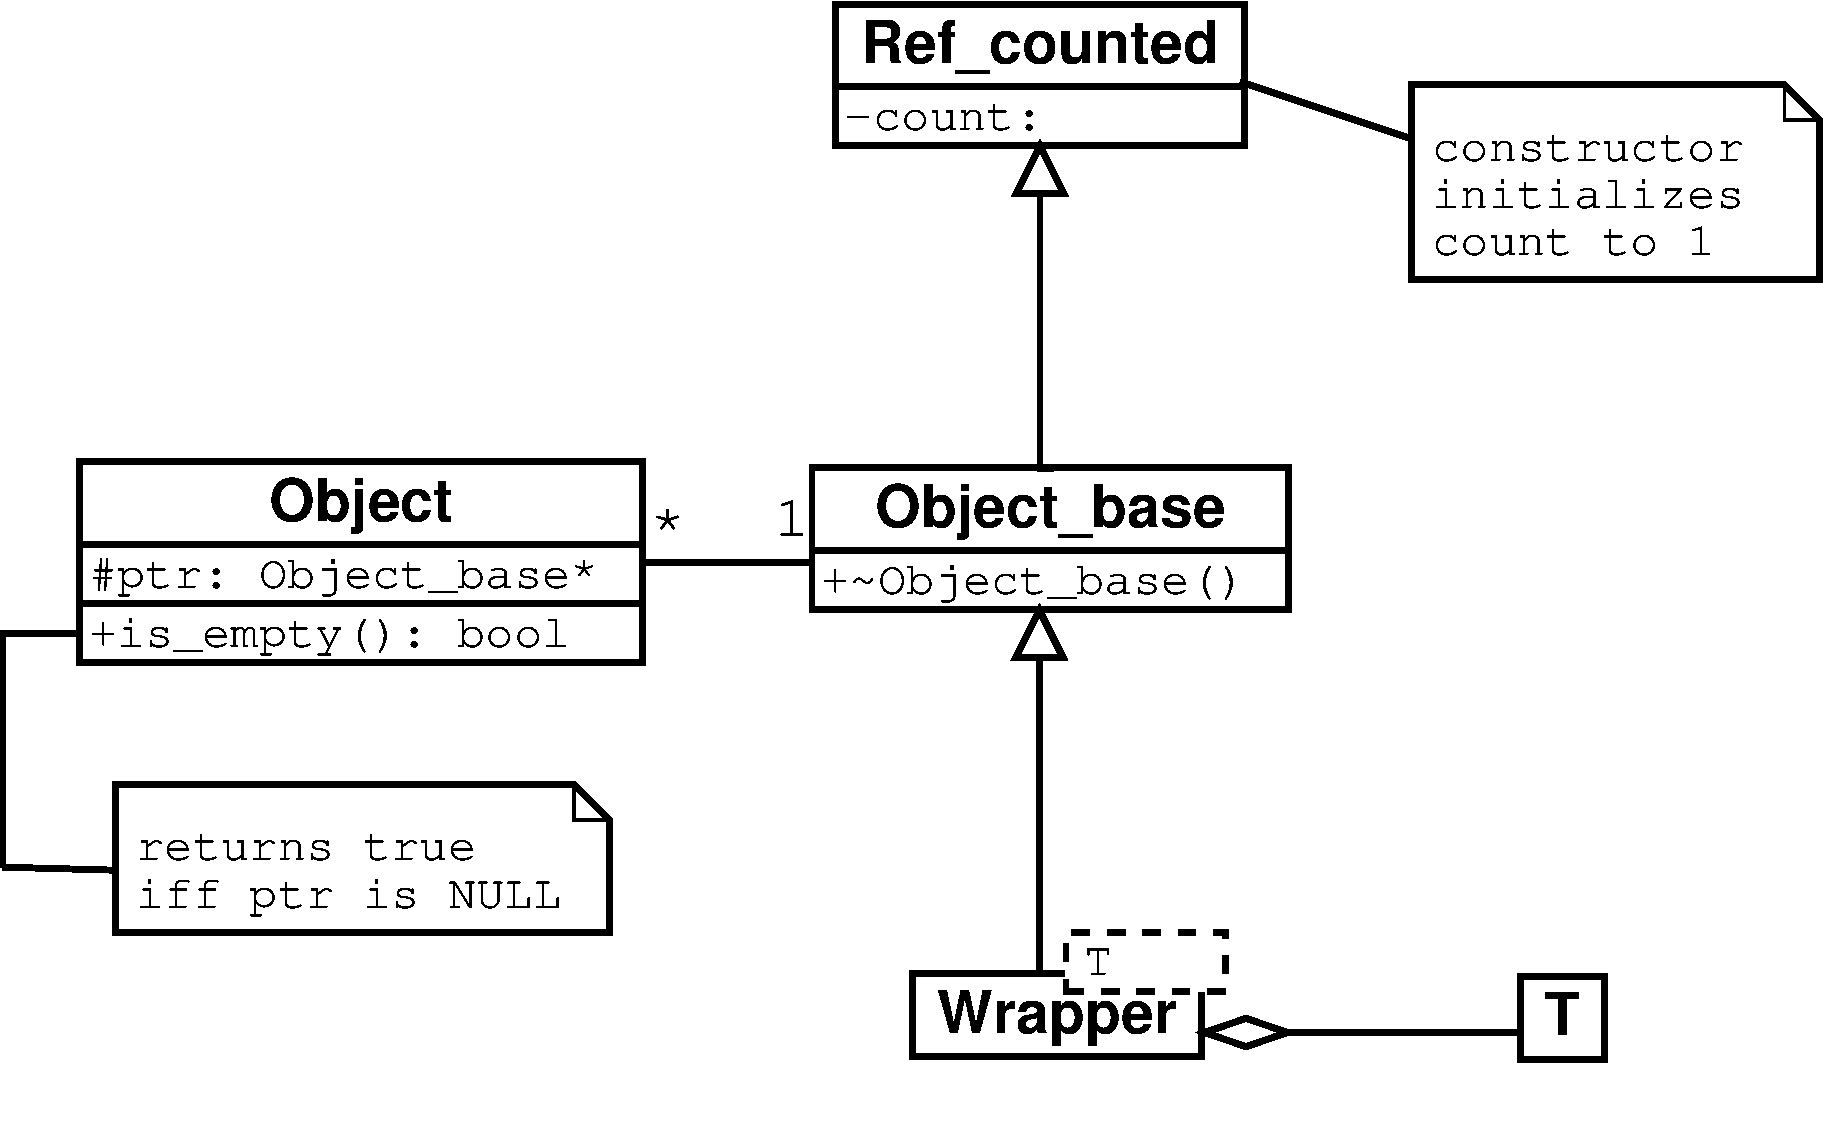
\includegraphics[width=11cm]{Developers_manual/fig/Object}
\end{center}
}
\caption{UML class diagram for faked object hierarchies (since 2.2-I-4).\label{Fig:Object}}
\lcRawHtml{
<CENTER>
<IMG BORDER=0 SRC="fig/Object.gif"
   ALT="Faked object heirarchies UML diagram"><BR>
</CENTER>
}
\end{figure}

Functions having a polymorphic return type create an object of the actual
result type and wrap it into an object of type \ccc{Object}.
Refer to the documentation of the 
\ccAnchor{http://www.cgal.org/Manual/latest/doc_html/cgal_manual/STL_Extension_ref/Class_Object.html}{\ccc{Object}}
class for more details.

An alternative is to use a class handling several output iterators at the same time such as the classes
\ccAnchor{http://www.cgal.org/Manual/latest/doc_html/cgal_manual/STL_Extension_ref/Class_Dispatch_output_iterator.html}{\ccc{Dispatch_output_iterator}}
and
\ccAnchor{http://www.cgal.org/Manual/latest/doc_html/cgal_manual/STL_Extension_ref/Class_Dispatch_or_drop_output_iterator.html}{\ccc{Dispatch_or_drop_output_iterator}}.
